\documentclass[12pt, a4paper]{article}

\usepackage[T2A]{fontenc}
\usepackage[utf8]{inputenc}
\usepackage[english,russian]{babel}
\usepackage[left = 1.5 cm, right = 1.5 cm, top = 2cm, bottom = 2 cm, bindingoffset = 0 cm]{geometry}
\usepackage{amsmath,amsfonts,amssymb,amsthm,mathtools}
\usepackage{wasysym}
\usepackage{float}

\usepackage{tikz}

\usepackage{graphicx}
\graphicspath{{pictures/}}
\DeclareGraphicsExtensions{.pdf,.png,.jpg}

\usepackage{alltt}

\begin{document}
\begin{titlepage}
\newpage

\begin{center}
Министерство образования и науки Российской Федерации \\
Федеральное государственное автономное образовательное
учреждение высшего образования \\
Национальный исследовательский Нижегородский государственный
университет им. Н.И. Лобачевского \\
Институт информационных технологий, математики и механики \\
\end{center}

\vspace{12em}

\begin{center}
\textsc{\textbf{Отчёт по лабораторной работе}}\\
\textsc{\textbf{Численные методы исследования динамических систем с помощью пакета MatLab}}
\end{center}

\vspace{14em}



\newbox{\lbox}
\savebox{\lbox}{\hbox{Барабаш Н. В.}}
\newlength{\maxl}
\setlength{\maxl}{\wd\lbox}
\hfill\parbox{11cm}{
\hspace*{5cm}\hspace*{-2cm} \textbf{Выполнил:} студент группы 381803-1 \\
\hspace*{5cm}\hspace*{-2cm} Петров Павел \\
\hspace*{5cm}\hspace*{-2cm} \textbf{Проверил:} научный сотрудник \\
\hspace*{5cm}\hspace*{-2cm} лаборатории динамического хаоса \\
\hspace*{5cm}\hspace*{-2cm} кафедры ТУиДС \\
\hspace*{5cm}\hspace*{-2cm} Казаков А. О. \\
\\
}


\vspace{\fill}
\vspace{\fill}

\begin{center}
Нижний Новгород \\2021
\end{center}

\end{titlepage}
\section{Аттрактор Лоренца}
Рассмотрим систему Лоренца и построим для неё бифуркационную диаграмму.
\begin{equation*}
	\begin{cases}
		\dot x = \sigma (y - x) \\
		\dot y = x(r - z) - y \\
		\dot z = xy - bz
	\end{cases}
\end{equation*}
$\sigma, \; r, \; b$ - положительные параметры.

Построим кривую $l_1$.
\newline
В Starter выберем момент времени $t=0$ и точку $(x,y,z) = (0.001, 0, 0)$. В Integrator выставим параметр interval в 2,5. Параметры - $(\sigma, r, b) = (10, 14, \frac{2}{3})$. Построим кривую. Далее выберем начальную точку как состояние равновесия: $\textbf{Type|Initial Point|Equilibrium}$, а кривую - $\textbf{Type|Curve|ConnectionSaddle}$. Нажмём $\textbf{Compute|Forward}$ и затем в Data Browser выберем HTHom Select Connection. После этого выбираем в Starter параметры (r, SParam1, eps1) и зануляем параметр SParam1. В Data Browser выбираем HTHom SParam1 equal to zero. Теперь выберем параметры (r, eps1, T) и будем занулять eps1. Выбираем в Data Browser HTHom eps1 small enough, а в initializer - Homoclinic to Saddle. Выбираем параметры (s, r, T) и начинаем строить кривую $l_1$.
\begin{figure}[H]
	\center{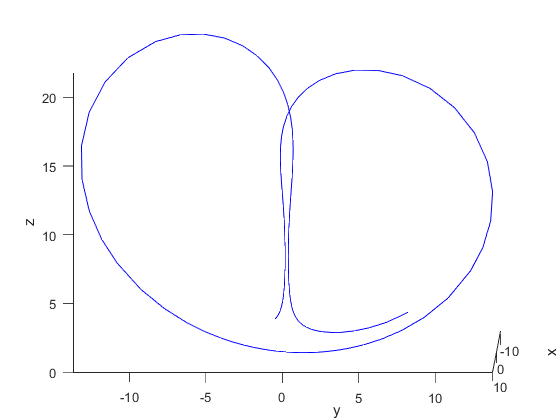
\includegraphics[scale=0.7]{LorenzLL1}}
	\caption{Выбор Connection Saddle}
\end{figure}
\begin{figure}[H]
	\center{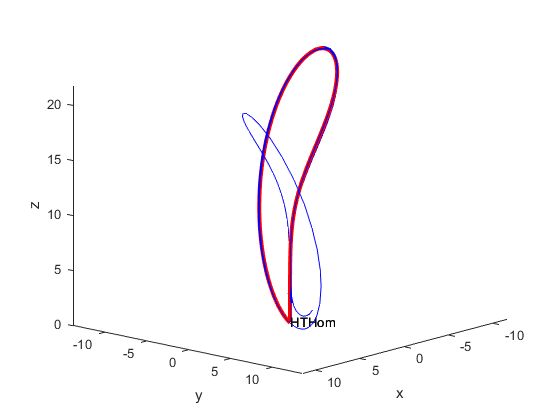
\includegraphics[scale=0.7]{LorenzLL12}}
	\caption{Зануляем SParam1 и eps1}
\end{figure}
\begin{figure}[H]
	\center{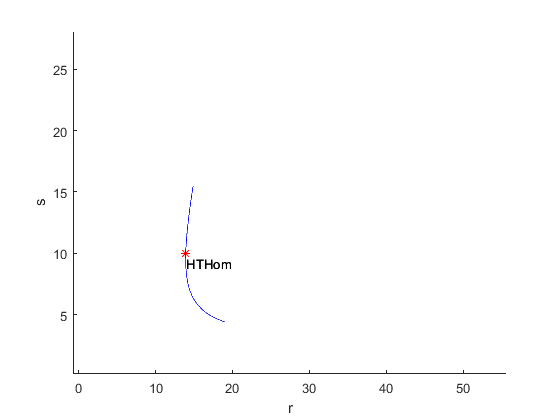
\includegraphics[scale=0.7]{LorenzLL13}}
	\caption{Кривая бифуркации вилка}
\end{figure}
Построим кривую $l_3$.
\newline
В Starter выберем момент времени $t=0$ и точку $(x,y,z) = (0.001, 0, 0)$. Параметры - $(\sigma, r, b) = (10, 2, \frac{2}{3})$ Найдём состояние равновесия и затем выберем эту точку как состояние равновесия: $\textbf{Type|Initial Point|Equilibrium}$. Протянем её по параметру $r$, пока не найдём точку Hopf. Выберем её в Initializer, выберем пункт Hopf (init\_H\_H), затем, протянув по двум параметрам $(\sigma, r)$, получим кривую $l_3$.
\begin{figure}[H]
	\center{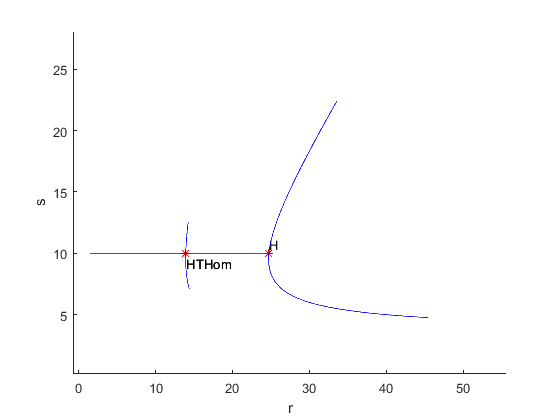
\includegraphics[scale=0.8]{lorenzl2}}
	\caption{Кривая бифуркации вилка}
\end{figure}
Построим кривую симметричной бифуркации вилки.
\newline
Для этого при тех же параметрах и начальной точке находим состояние равновесия, затем протягиваем его по r в сторону уменьшения, пока не наткнёмся на Branch Point. Выберем эту точку в Data Browser, а в Initializer выберем Equilibrium (BP). Далее протягиваем бифуркационную кривую по параметру $\sigma$.
\begin{figure}[H]
	\center{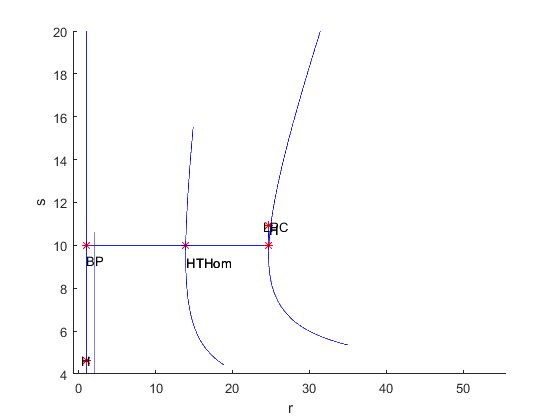
\includegraphics[scale=0.8]{LorenzLL14}}
	\caption{Кривая бифуркации вилка}
\end{figure}
\end{document}